\subsection{Controller}

\begin{figure}[h!]
	\centering
 	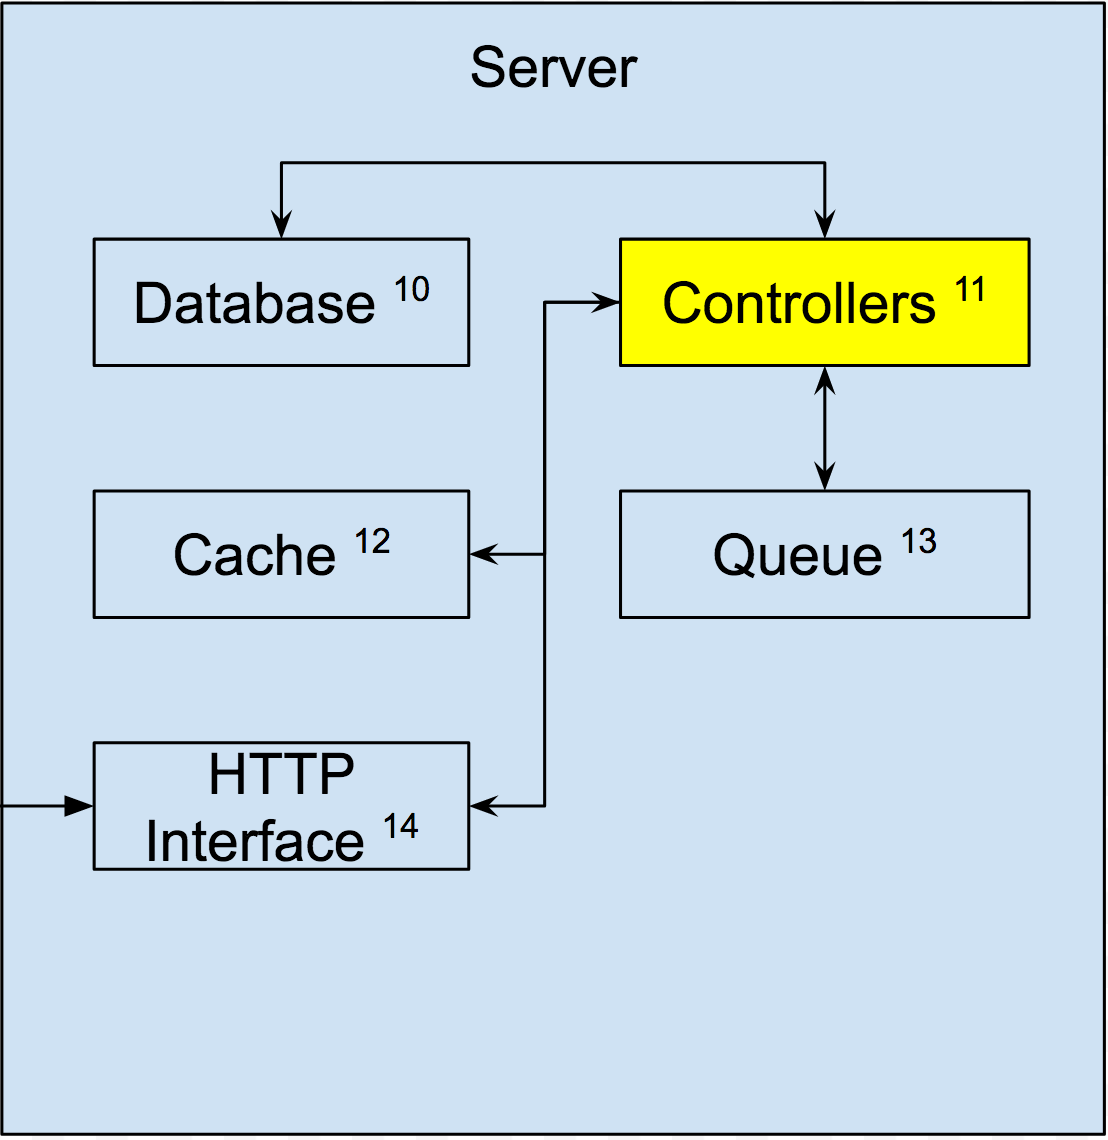
\includegraphics[width=0.60\textwidth]{detailed-design-specification-latex/images/server/server_controller.png}
 \caption{}
\end{figure}

\newpage

\subsubsection{Subsystem Operating System}
This project is primarily software, but we will be hosting our live site using Heroku, so whatever OS they are using for their servers (usually UNIX systems such as macOS, Linux) is our OS. \\

\subsubsection{Subsystem Software Dependencies}
Libraries \\
- Gorilla Mux \\

\subsubsection{Subsystem Programming Languages}
The programming language to be used will be Go. Go is a modern and great programming language to work with and will satisfy our needs to provide an implementation of controller methods.

\subsubsection{Subsystem Data Structures}
The primary data structures that will be returned from the controller will be hash maps and arrays. Internally, the controller will use structs (similar to objects in Object Oriented Programming languages) and arrays.

\subsubsection{Subsystem Data Processing}
To maintain authentication, we use a strategy where we read in each requests header to verify that the user has valid and non-expired token. A token in this context will either allow the user to access the requested resources or direct them to re-authorize. Afterwards, we validate the user has sent in a valid JSON object, and convert it to a map in Go.

\newpage
